Regarding the hardware used in this project, Figure~\ref{fig:circuit} shows a complete overview of which elements have been used and how they were connected.
\begin{figure}[h]
    \centering
    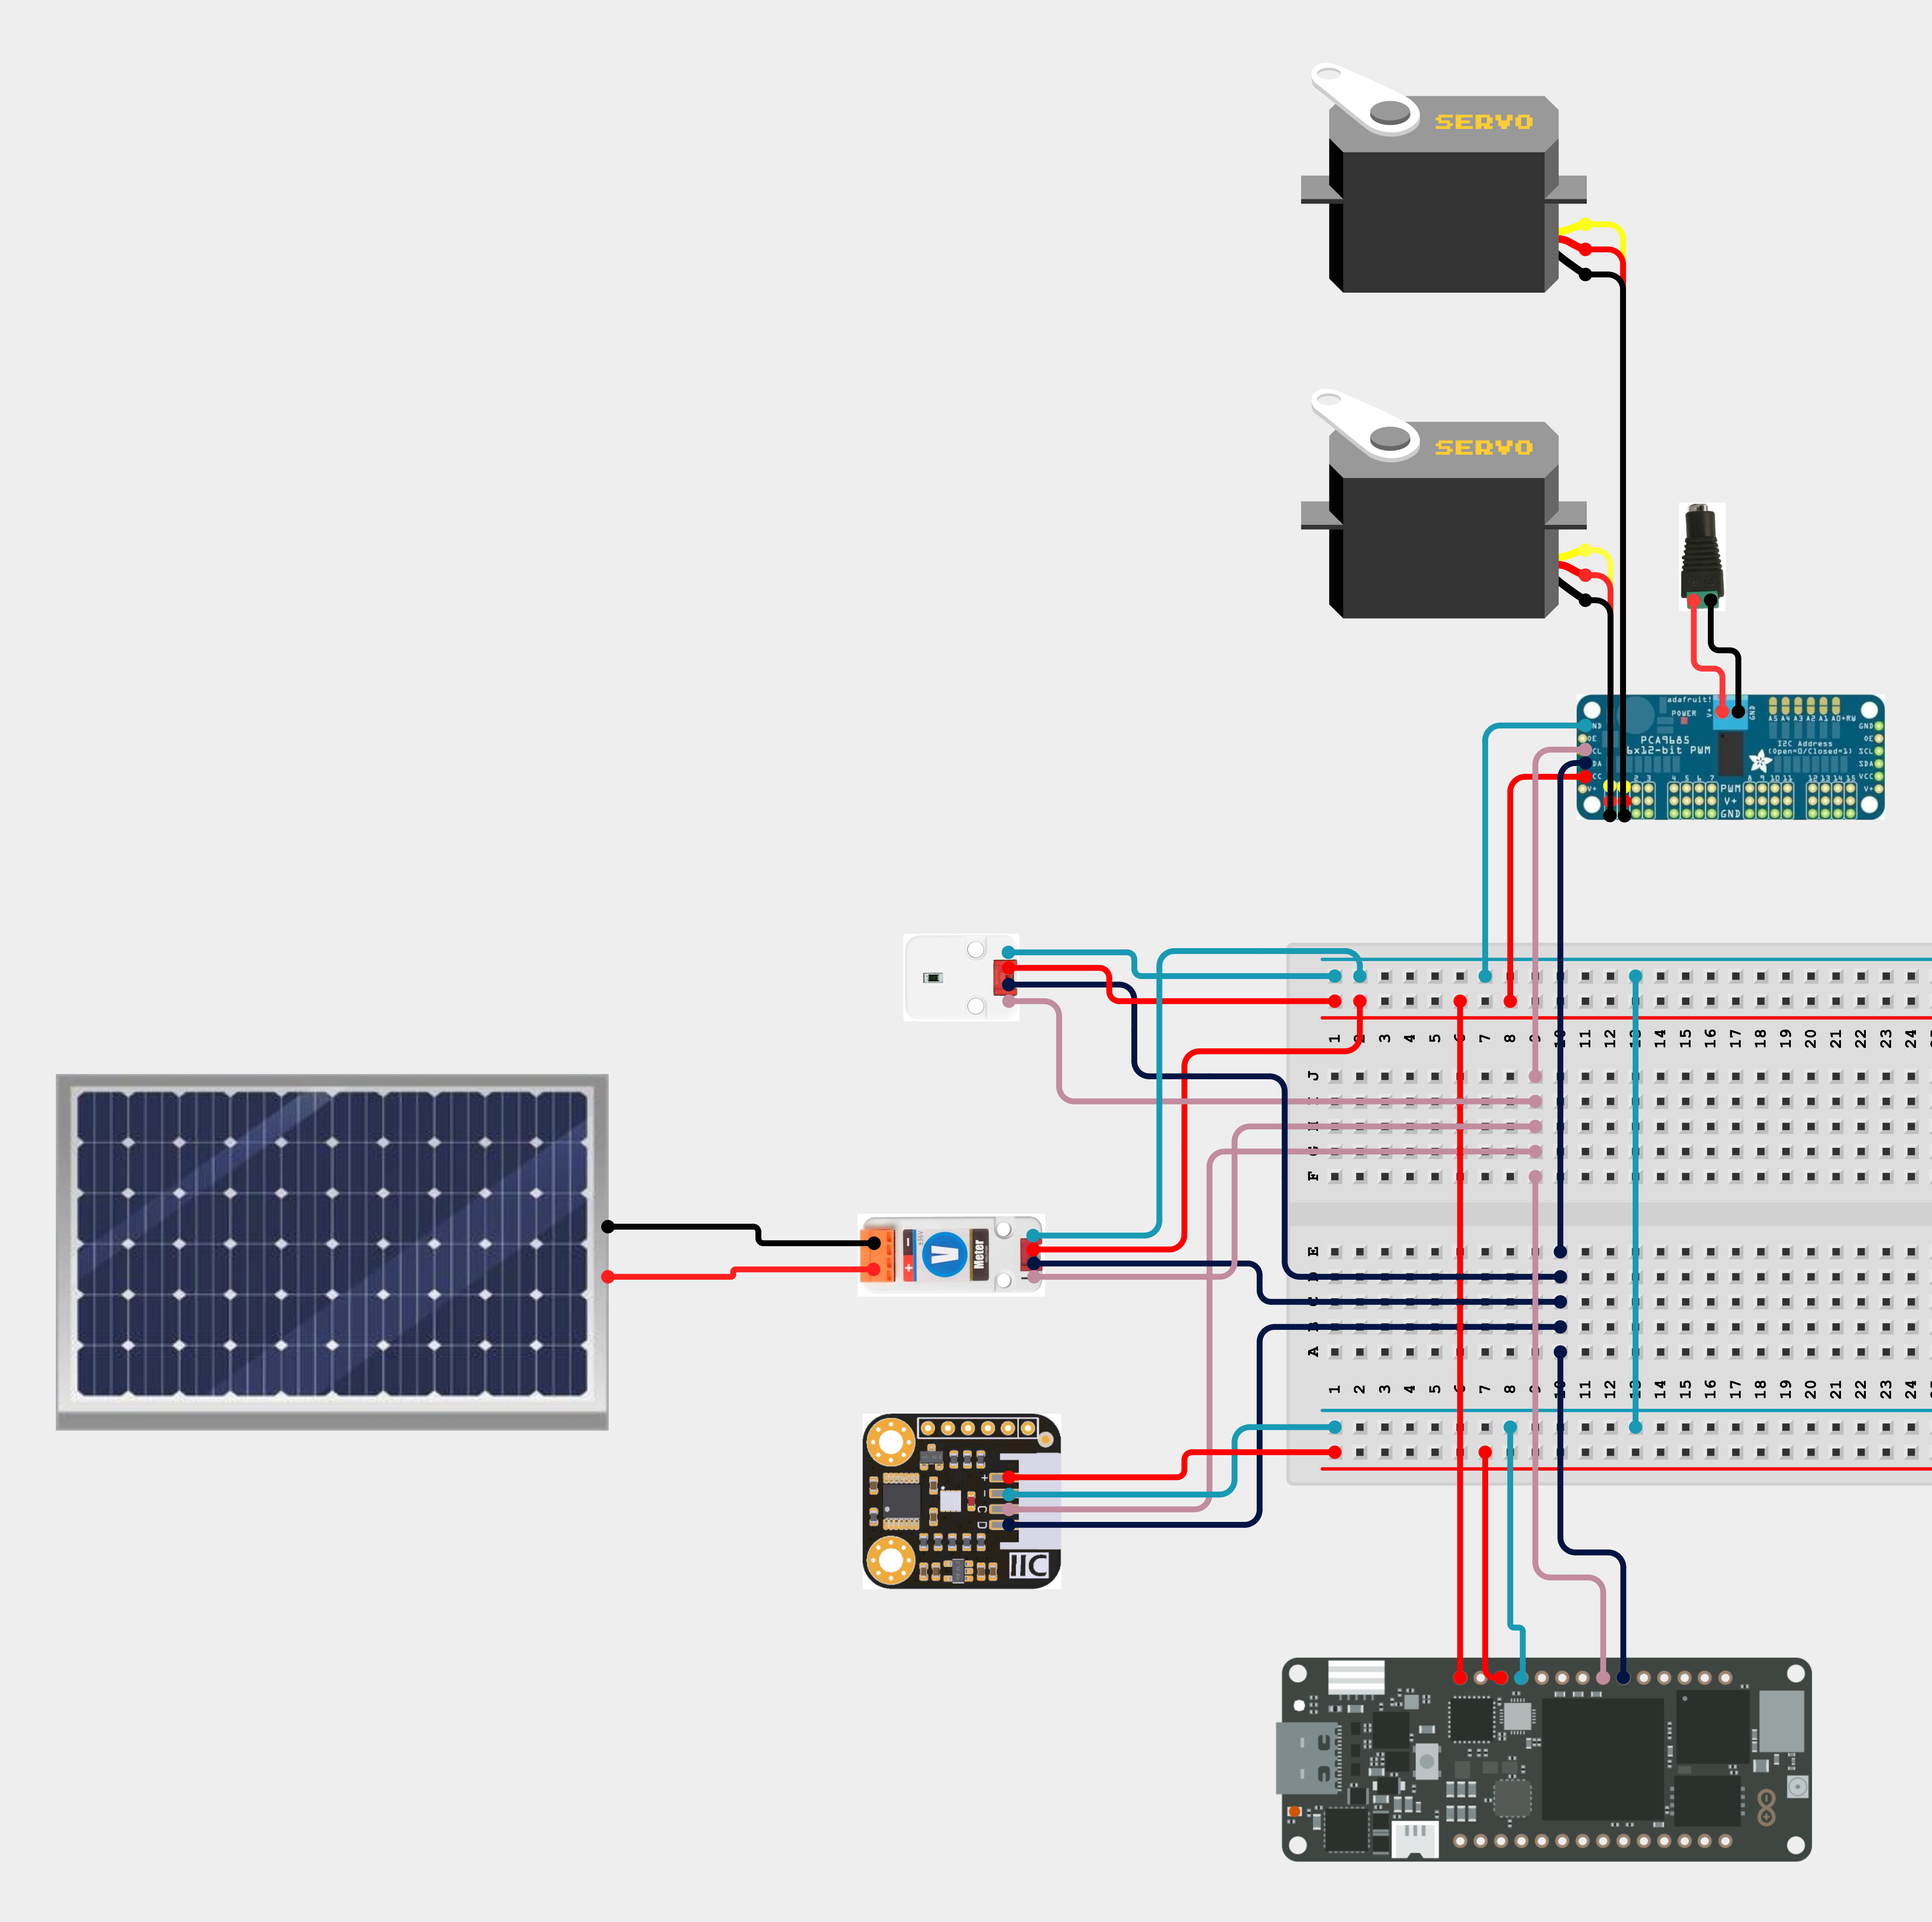
\includegraphics[width=10cm]{../assets/png/project-circuit}
    \caption{Overview of the hardware used in our project.}
    \label{fig:circuit}
\end{figure}
The parts used where: two servos, a motor shield, a light intensity sensor, a
voltmeter connected to a solar panel, an ambient sensor, and an Arduino Portenta
H7. All the components were connected to the Portenta board using the I2C
protocol. Please note that our delivered code, available in
\texttt{src/arduino/arduino.ino}, has been well commented and cleaned up. Setup
and loop code is well separated in the two homonoymous methods.

\subsection*{Servos}
The two servos are the responsible for the movement of the solar panel. These
are high-torque servos and are attached to a 3D-printed structure that holds the
solar panel and moves it on two different planes. The bottom servo rotates the
panel, while the top servo adjusts the inclination of the panel. \\ \\
To be able to interface with the Arduino board, we used a motor shield to which we connected both servos.
Since they require some energy, the shield was connected to the wall outlet by means of a power supply cable. \\ \\
This is our control algorithm for moving the servos in the best position:

\begin{lstlisting}[style=mystyle,language=C,caption={The \texttt{get\_direction} function keeps track of the 2 rotation axis and computes the direction.}]
// Initiate values and start servos movement loop
int best_servo_1 = 200;
int best_servo_2 = 300;
float curr_tension = read_tension();

// Perform scan only if current tension is < 95% of the last best tension, and it is daytime (tension > 0.15)
if ((curr_tension < 0.95 * max_value || max_value == 0) && curr_tension > 0.15) {
    max_value = 0.0;

    for (int angle = angle_min_1; angle <= angle_max_1; angle += ANGLE_INCREASE) {
        int pulse = map(angle, 0, 360, SERVOMIN, SERVOMAX);

        // Move bottom servo
        pwm.setPWM(SERVO_1, 0, pulse);

        for (int angle_2 = angle_min_2; angle_2 <= angle_max_2; angle_2 += ANGLE_INCREASE) {
            int pulse = map(angle_2, 0, 500, SERVOMIN, SERVOMAX);

            // Move top servo
            pwm.setPWM(SERVO_2, 0, pulse);
            delay(100);

            float current = read_tension();

            if (current > max_value) {
                best_servo_1 = angle;
                best_servo_2 = angle_2;
                max_value = current;
            }

            delay(500);
        }
    }

    angle_min_1 = best_servo_1 - ANGLE_INCREASE * 2;
    angle_max_1 = best_servo_1 + ANGLE_INCREASE * 2;

    int pulse1 = map(best_servo_1, 0, 360, SERVOMIN, SERVOMAX);
    int pulse2 = map(best_servo_2, 0, 360, SERVOMIN, SERVOMAX);

    // Move servos to best found position
    pwm.setPWM(SERVO_1, 0, pulse1);
    pwm.setPWM(SERVO_2, 0, pulse2);
}
\end{lstlisting}

As part of the telemetry data, we also added a small piece of code that keeps
track of the orientation (NW = nord west, SO = south ovest, etc.). The IoT Solar
Station should be positioned initially toward the north direction, since it is a
closed-loop control algorithm for simplicity.

\begin{lstlisting}[style=mystyle,language=C,caption={The \texttt{get\_direction} function keeps track of the 2 rotation axis and computes the direction.}]
String get_direction(int servo_0, int servo_1) {
    String direction = "N";

    float tolerance = 115;
    float inclinations[3] = {300, 580, 640};
    float directions[4] = {150, 265, 380, 495};

    if (servo_0 >= directions[0] - tolerance && servo_0 <= directions[0] + tolerance) {
        direction = "N";
    } else if (servo_0 > directions[1] - tolerance && servo_0 <= directions[1] + tolerance) {
        direction = "NW";
    } else if (servo_0 > directions[2] - tolerance && servo_0 <= directions[2] + tolerance) {
        direction = "W";
    } else if (servo_0 > directions[3] - tolerance && servo_0 <= directions[3] + tolerance) {
        direction = "SW";
    }

    if (direction == "N" && servo_1 > inclinations[1]) {
        direction = "S";
    } else if (direction == "NW" && servo_1 > inclinations[1]) {
        direction = "SE";
    } else if (direction == "W" && servo_1 > inclinations[1]) {
        direction = "E";
    } else if (direction == "SW" && servo_1 > inclinations[1]) {
        direction = "NE";
    }

    return direction;
}
\end{lstlisting}

\subsection*{Ambient Sensor}
Attached to the system, there is an ambient sensor which will capture several
different measurements. These measurements are temperature, pressure, humidity,
and light intensity. These measurements are not used to drive the
best-position-seeking algorithm for the solar panel, but are used to populate
the weather station's dashboard.

\subsection*{Light Intensity Sensor}
As with the ambient sensor, the light intensity sensor does not serve a real
purpose towards the computation of the best position. The data taken from this
sensor is used in the weather station dashboard.

\subsection*{Voltmeter}

The system must actively adjust the solar panel in response to the position of
the sun, adjusting its position to maximize energy absorption. This is done with
two main actions, searching for the optimal position and scanning the various
positions and angles. \\ \\
Our model must also take into account times of low solar intensity such as
cloudy conditions or night. In these scenarios, our system enters an
energy-saving phase. The system will only capture sensor data, and as long as
the produced voltage does not exceed 1V, the system will not search for new
positions (Figure~\ref{fig:seros-sm}).
\begin{figure}[h]
    \centering
    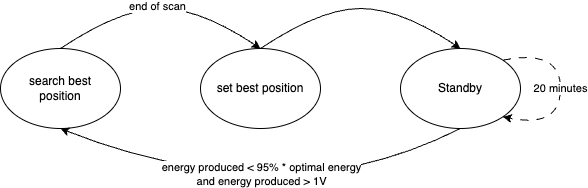
\includegraphics[width=12cm]{../assets/png/servos-state-machine}
    \caption{State machine that describes the lifecycle of our system.}
    \label{fig:seros-sm}
\end{figure}
